\documentclass[fleqn]{article}
\oddsidemargin 0.0in
\textwidth 6.0in
\thispagestyle{empty}
\usepackage{import}
\usepackage{amsmath}
\usepackage[backend=bibtex]{biblatex}
\usepackage[utf8]{inputenc}
\usepackage{csquotes}
\usepackage{graphicx}
\usepackage{flexisym}
\usepackage{calligra}
\usepackage{amssymb}
\usepackage{bigints} 
\usepackage[english]{babel}
\usepackage{float}
\usepackage[colorinlistoftodos]{todonotes}
\usepackage{blindtext}
\usepackage{hyperref}

\addbibresource{references.bib}

\hypersetup{
  colorlinks=true,
  linkcolor=blue,
  filecolor=magenta,      
  urlcolor=cyan,
  pdfpagemode=FullScreen
}

\DeclareMathAlphabet{\mathcalligra}{T1}{calligra}{m}{n}
\DeclareFontShape{T1}{calligra}{m}{n}{<->s*[2.2]callig15}{}
\newcommand{\scriptr}{\mathcalligra{r}\,}
\newcommand{\boldscriptr}{\pmb{\mathcalligra{r}}\,}


\setlength{\arrayrulewidth}{0.5mm}
\setlength{\tabcolsep}{18pt}
\renewcommand{\arraystretch}{1.5}

\definecolor{hwColor}{HTML}{AD53BA}

\begin{document}

  \begin{titlepage}

    \newcommand{\HRule}{\rule{\linewidth}{0.5mm}}

    \center

    \begin{center}
      
\includegraphics[height=11cm, width=11cm]{asu.png}
    \end{center}

    \vline

    \textsc{\LARGE Advanced Laboratory I}\\[1.5cm]

    \HRule \\[0.5cm]
    { \huge \bfseries Zeeman Effect}\\[0.4cm] 
    \HRule \\[1.0cm]

    \textbf{Behnam Amiri}

    \bigbreak

    \textbf{Prof: Ralph Chamberlin}

    \bigbreak

    \textbf{Lab Partners: Daniel Henningsen, Micah Smith, Srihari Ravi}

    \bigbreak

    \textbf{{\large \today}\\[2cm]}

    \vfill

  \end{titlepage}

  \textbf{Abstract}
  \vspace{10px}

  This lab report represents the experimental procedure we did to learn about the Zeeman effect which is basically about 
  the splitting of a spectral line into several components through magnetic field or in other words, we had the magnetic field 
  interacting with electron. All the presented pictures in this lab report are from our own experiment.
  \vspace{10px}

  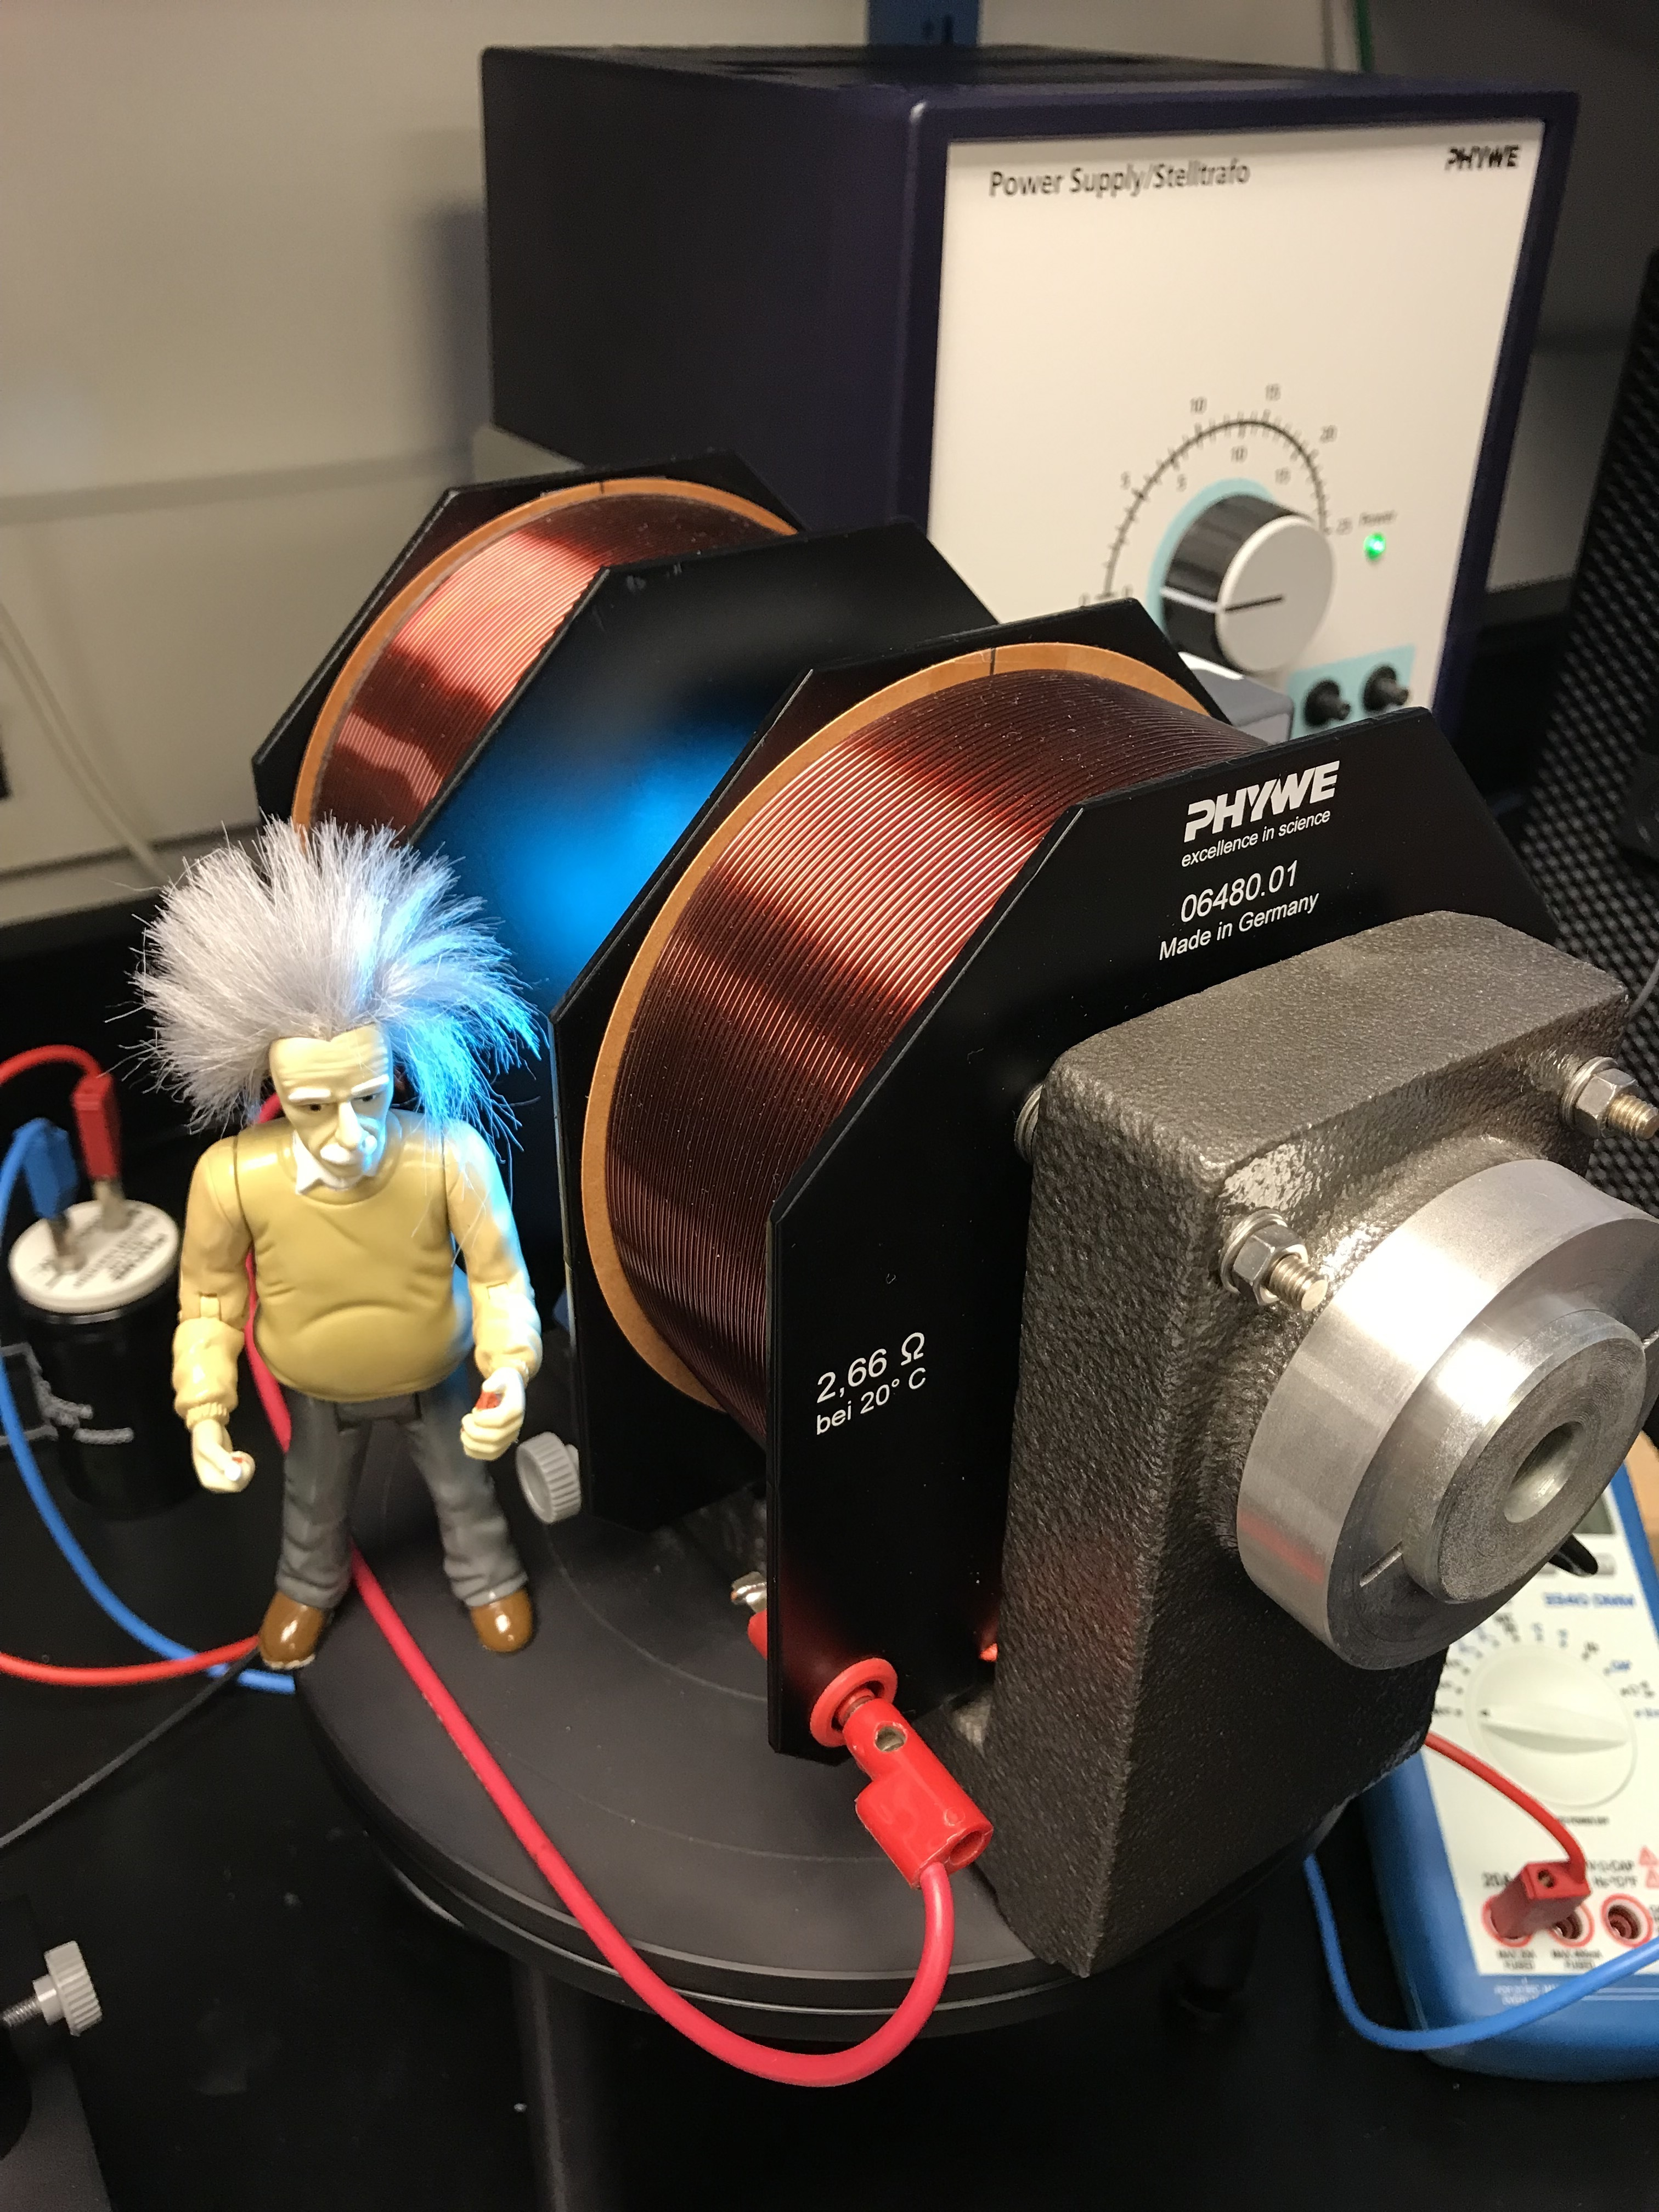
\includegraphics[height=12cm, width=12cm]{1.jpg}

  \vspace{20px}

  \textbf{II. Background Information}

  \vspace{10px}

  Magnetic fields effect how light behaves. The reason we study the Zeeman effect is that it has helped physicists to study the energy levels
  in atoms which is a very important topic in Quantum Physics.
  "In the late 1800s, Dutch physicist Pieter Zeeman made discovered that powerful magnetic currents would widen the convergences of units 
  of sodium under intense heat which is known is the Zeeman effect or \textbf{anomalous Zeeman effect}." \textcite{One}

  \vspace{20px}

  \textbf{I. Introduction}

  \vspace{10px}

  Zeeman effect has to do with an atom in a magnetic field. As it was mentioned, It was discovered by a Dutch physicist Pieter Zeeman who lived
  from 1865 to 1943. He received the second physics nobel prize for "recognition of the extraordinary service they rendered by their researches into 
  the influence of magnetism upon radiation phenomena" in 1902. \textcite{Two} The work was actually done in 1896 at a time where there was a 
  very little idea of qunatum to be. He discovered that the spectral lines seemed to \emph{split the in the magnetic field.} It is an almost 110 years 
  old result, therefore its explanation and understanding took about some decades because they could not do it without quantum mechanics. Therefore,
  nobody could figure our what had happened but was a very important result in its time.
  
  Zeeman effect still remains very important. In fact it is used nowadays in studies of astrophysics, the sunspots. The sunspots are the places 
  in the sun where the temprature is a litte lower. Those are places where the magnetic fields lines in the sun sort of breakout from the 
  interior to the exterior. Scientists can measure the magnetic fields of the sun with the help of the Zeeman effect. \textcite{Three}   

  \vspace{20px}

  \textbf{III. Theory}

  \vspace{10px}

  The spin of the electron around the nucleus of the atom creates the electron's magnetic dipole moment $\mu$. Basically the electron spins 
  around the nucleus and the fact that electron has a negative charge creates magnetic dipole $\mu$ that points perpendicular with respect to
  the area that is circumscribed by the spin of that electron. If we take that atom and place it inside an external magnetic field $\overrightarrow{B}$
  then (for example) along the $z$ axis then the magnetic field $\overrightarrow{B}$ will create a torque that will act on the magnetic field dipole to orient
  along the same exact axis. Magnetic dipole moment along the $z$ axis is:
  $$
    \mu_z=\mu_B \bullet m_l
  $$

  Where $\mu_B$ is Bohr magneton which its magnitude is $\dfrac{e \hbar}{2 m_e} \approx 5.79 \times 10^{-11} ~ MeV/T$ \textcite{Four} and $m_l$ is magnetic quantum number. The Zeeman effect is basically caused by the magnetic dipole 
  moment of that electron. Once again if we take that atom and place it inside of an external magnetic field $\overrightarrow{B}$, then 
  certain orbital of that atom will undergo \textbf{spectral splitting} (they split into different energy levels). Note that not all
  orbitals of that atom have the ability to undergo the energy splitting. Number of energy splits of any orbital depends on the orbital quantum $L$ that is given by $2\ell+1$ where $\ell$ is the orbital quantum 
  number of that electron inside of that atom.

  Why exactly does the spectral splitting occur? We know that an electron has magnetic dipole moment $\mu$. When it is placed into 
  $\overrightarrow{B}$, the torque acts on $\mu$ works to orient that electron's $\mu$ along the same direction as the magnetic fields.


  \vspace{20px}

  \textbf{IV. Experimental Procedure}

  \vspace{10px}

  We just followed the given steps in the
  lab document. First off, we learned about the equipment used in the experiment followed by the inital steps provided to us by 
  Prof.Chamberlin. It was very interesting to see how the power supply and the magnetic field strength was affecting the interference 
  of a light beam. \textcite{Five}

  \vspace{20px}

  \textbf{V. Results}

  \vspace{10px}

  We have the following results from the experiment. Please refer to the description of each plot for details.

  \vspace{20px}

  \begin{figure}[h!]
    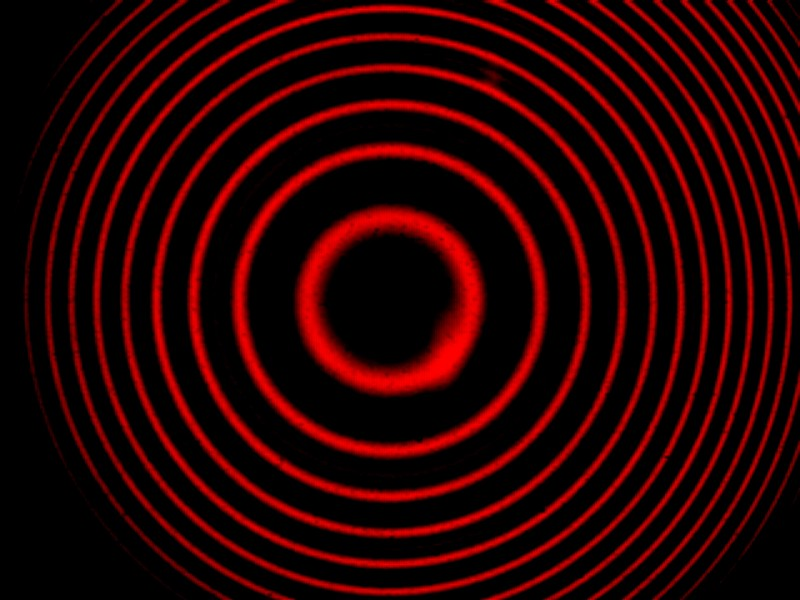
\includegraphics[height=7cm, width=9cm]{Second.jpg}
    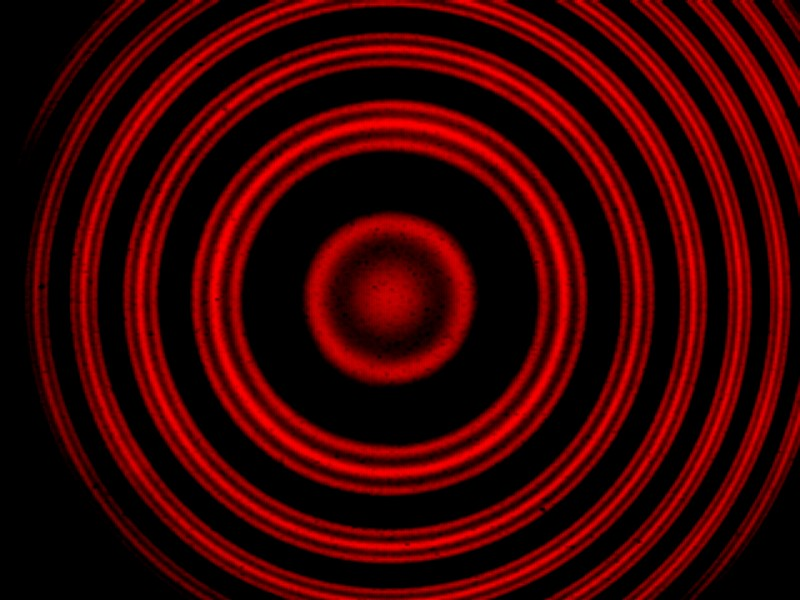
\includegraphics[height=7cm, width=9cm]{First.jpg}
    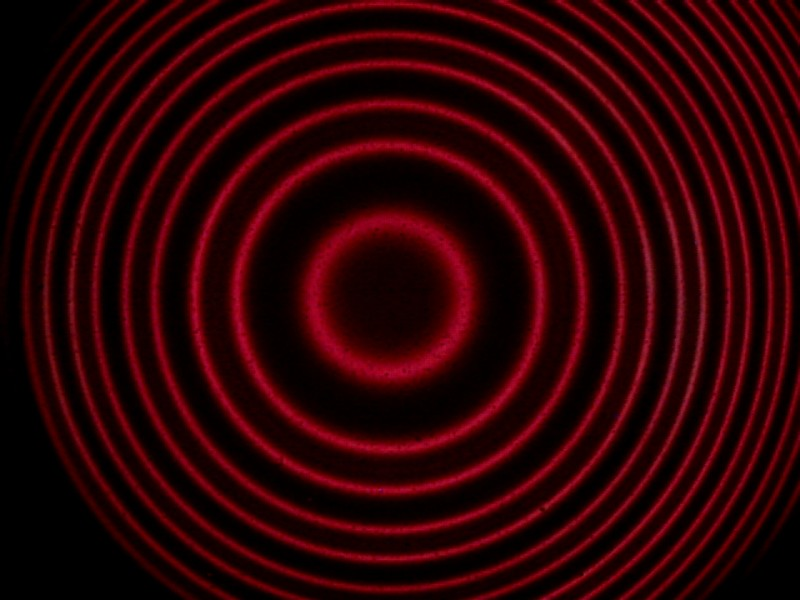
\includegraphics[height=7cm, width=9cm]{Third.jpg}
    \caption{xxx}
  \end{figure}

  \pagebreak


  \begin{figure}[h!]
    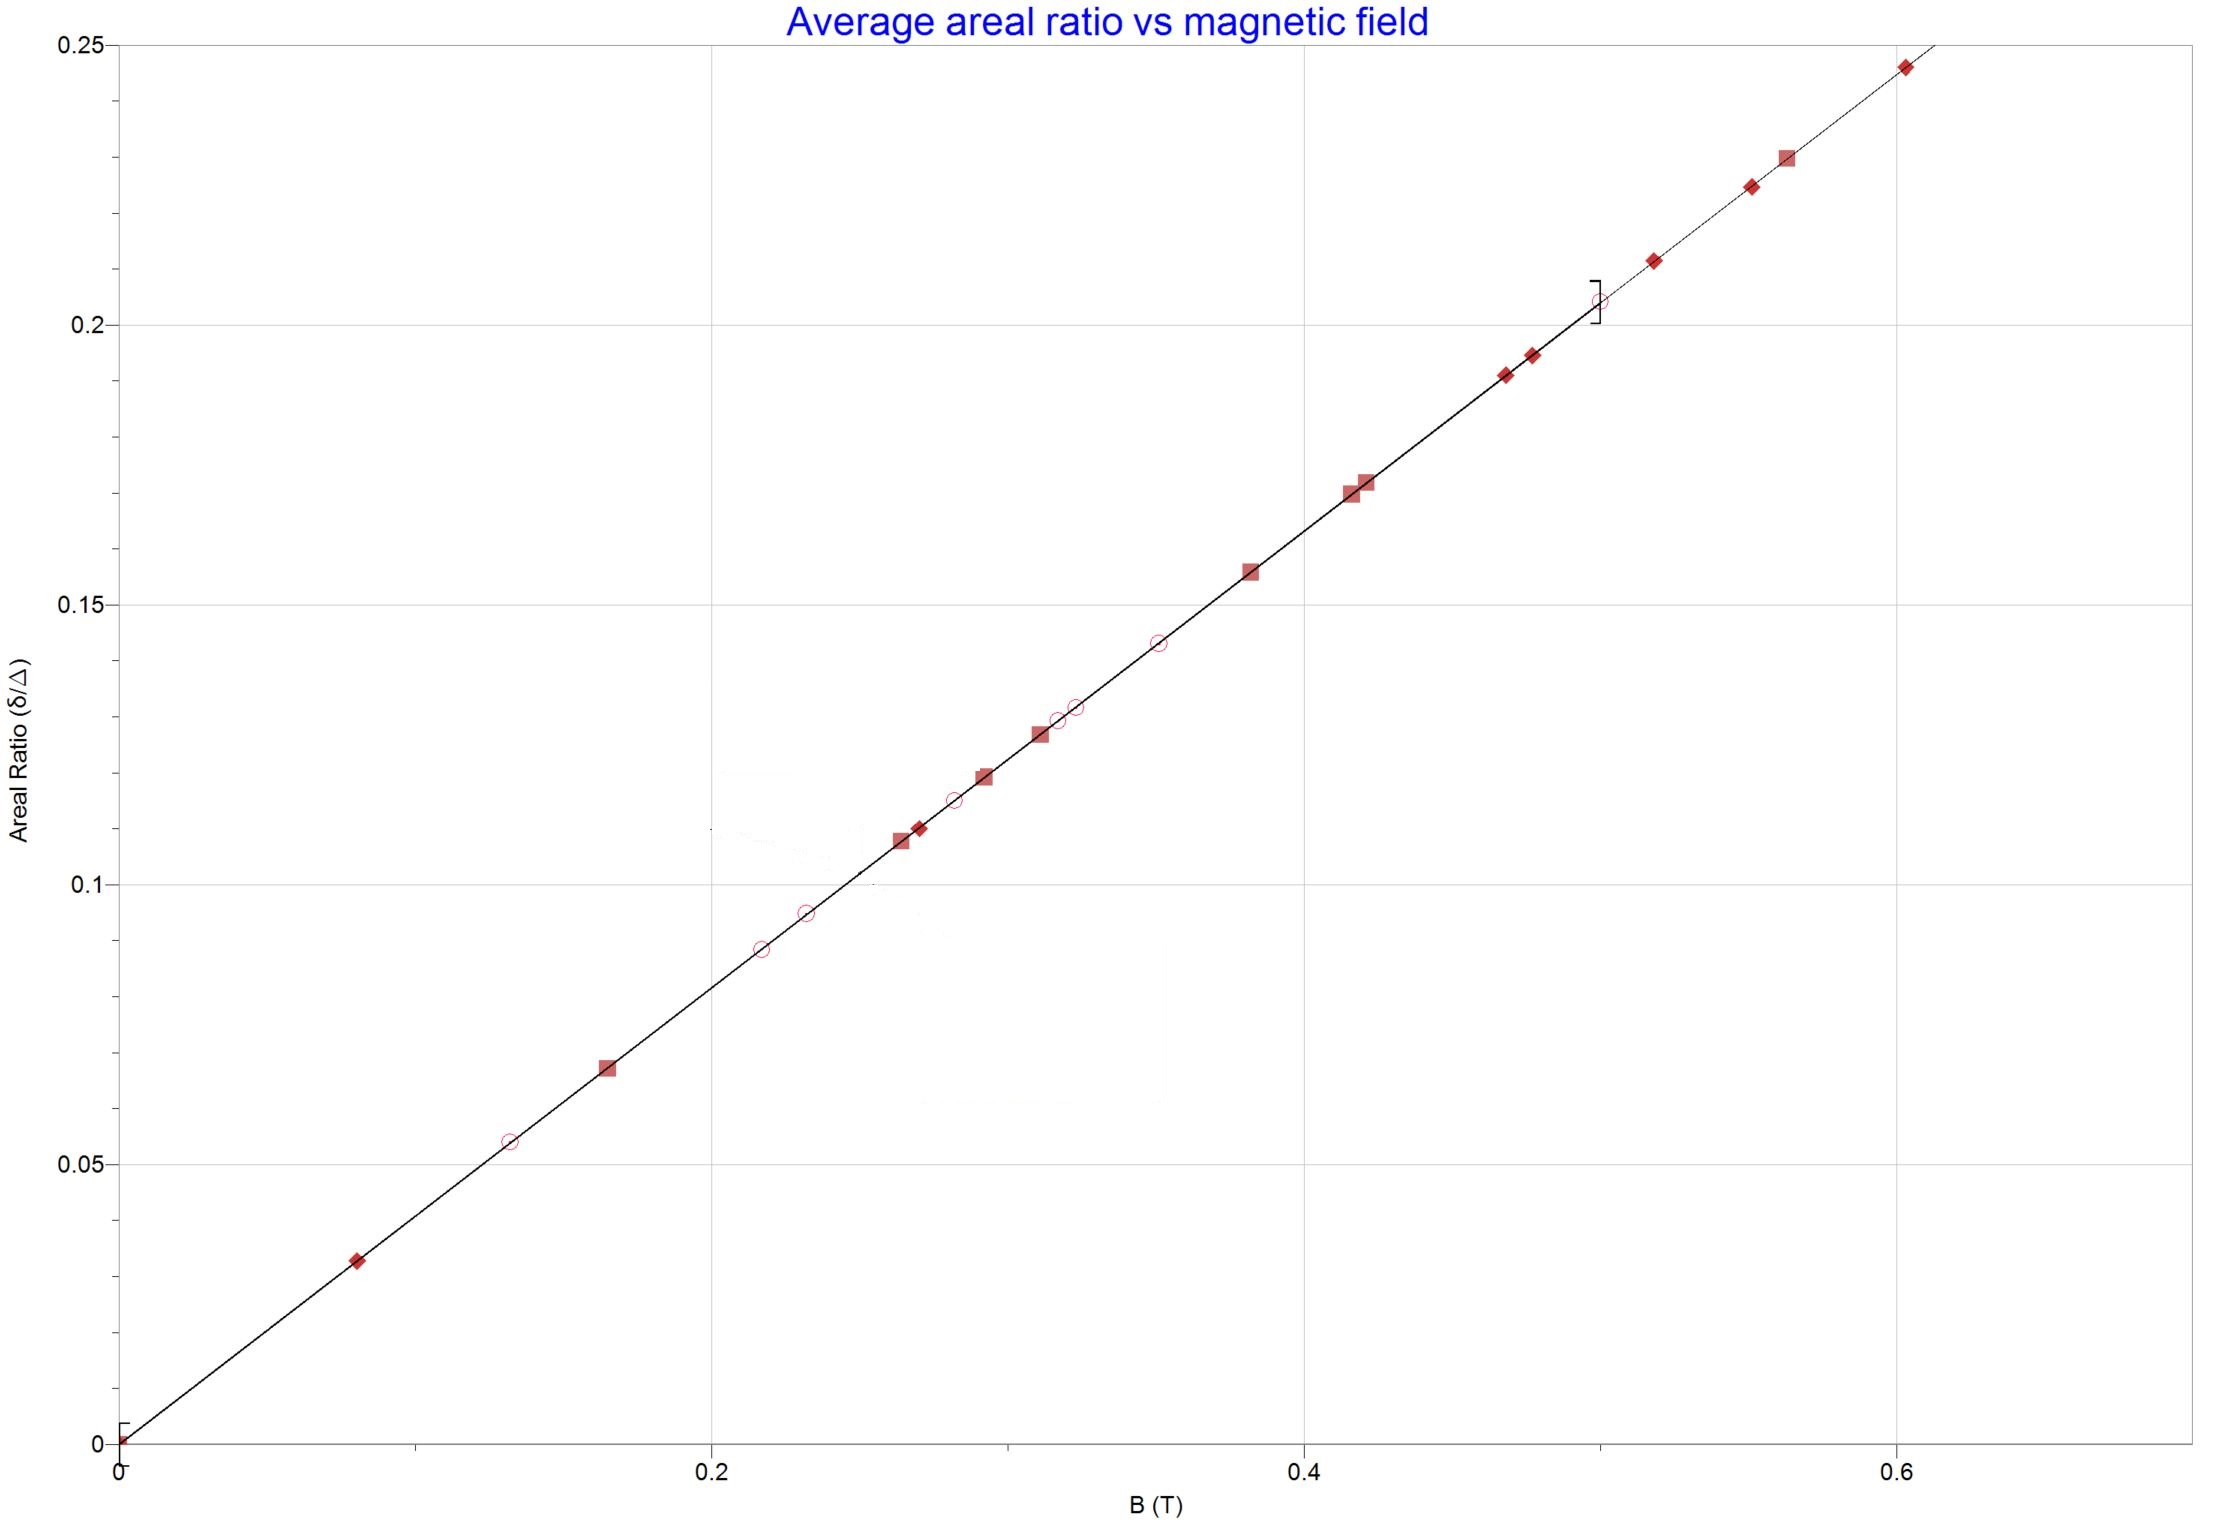
\includegraphics[height=14cm, width=16cm]{Figure2.JPG}
    \caption{xx}
  \end{figure}

  \pagebreak

  \begin{figure}[h!]
    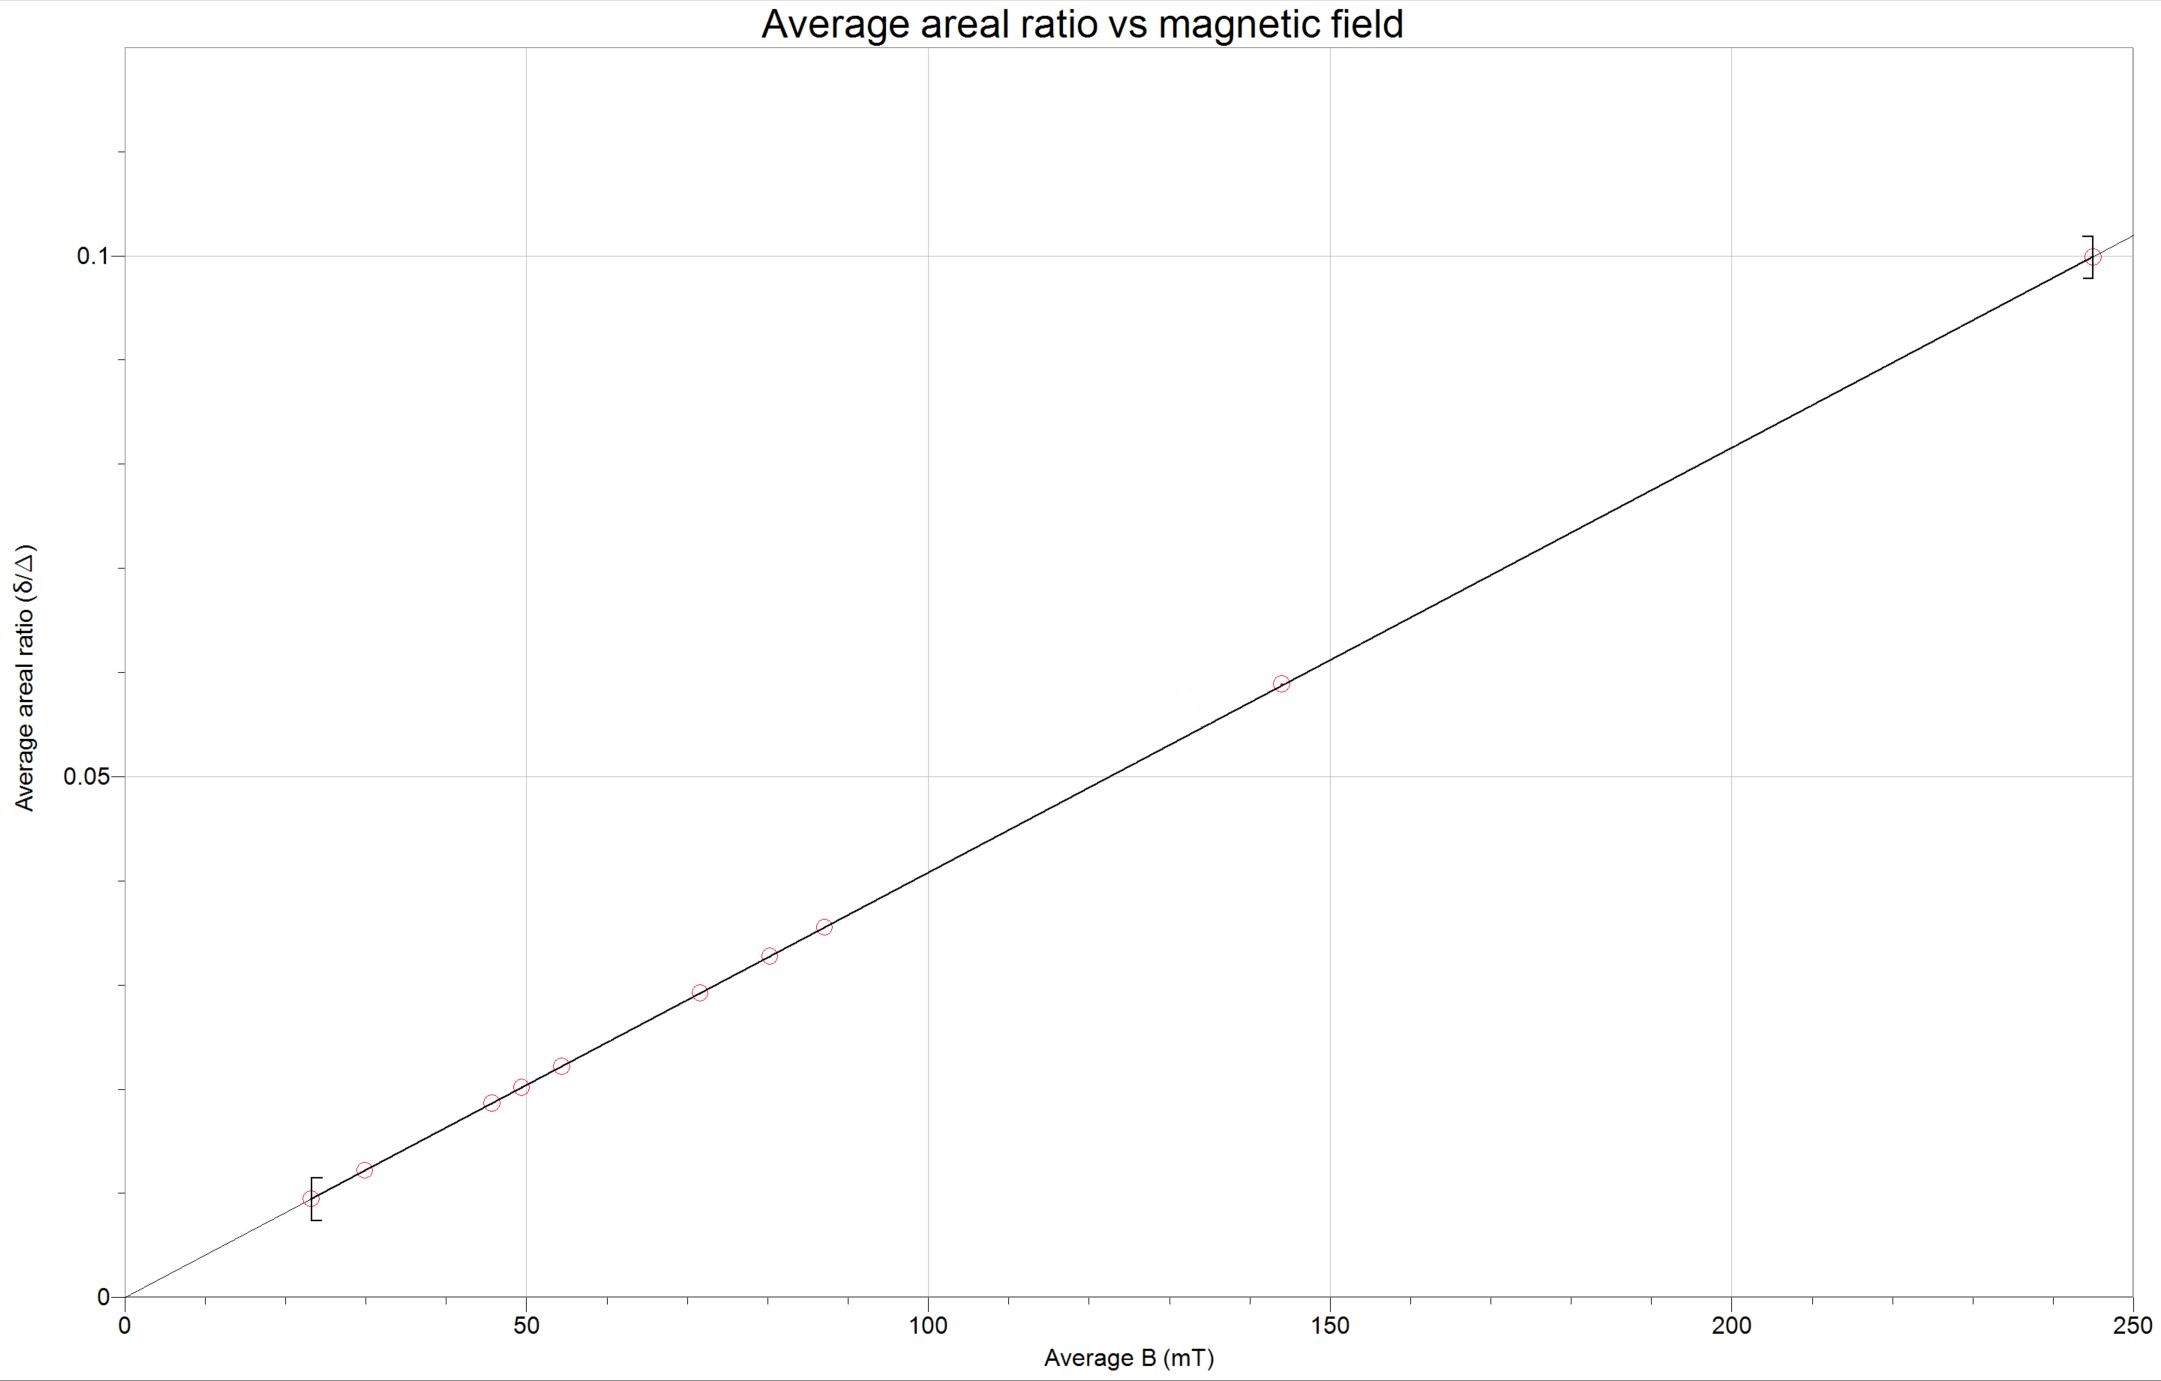
\includegraphics[height=14cm, width=16cm]{Figure3.JPG}
    \caption{xxx}
  \end{figure}


  \pagebreak

  \textbf{VI. Discussion}

  \vspace{10px}

  It was observed that when the magnetic field is increased, each ring in the interference splits into three rings and as s result a line
  triplet is created. One ring remains unchanged but the other two rings are located at the same distance with a small radius further 
  inside and the smaller radius further outside. By putting the polarization filter into the beam path (perpendicular to the magnetic field)
  then only the two split rings are observed. And if the polarization is parallel to the magnetic field then the original ring is there. Hence,
  the light of the three rings is linearly polarized.

  By rotating the electromagnet source by $90^{\circ}$ and observe the light longitudinally like parallel to the magentic field. Now by 
  increasing the magnetic field strength we can observe that each ring in the interference image splits into 2 rings. What happens here 
  is that the original ring disappears while the other two rings exist.

  $\delta/\Delta$


  \vspace{20px}

  \textbf{VII. Conclusions}

  \printbibliography
\end{document}